\documentclass{article}

\newcommand{\ep}{\rule{.06in}{.1in}}
\textheight 9.5in

\usepackage{amssymb, bm}
\usepackage{amsmath}
\usepackage{amsthm}
\usepackage{graphicx, subcaption, booktabs}
\graphicspath{{/Users/andrewwork/thesis/jump-velocity/plots/}}

\usepackage{tikz, pgfplots, pgfplotstable, chemfig, xcolor}

% \usepgfplotslibrary{colorbrewer, statistics}
% \pgfplotsset{
%   exact axis/.style={grid=major, minor tick num=4, xlabel=$v^*$,
%     legend entries={PDF, CDF},},
%   every axis plot post/.append style={thick},
%   table/search
%   path={/Users/andrewwork/thesis/jump-velocity/dat-files},
%   colormap/YlGnBu,
%   cycle list/Set1-5,
%   legend style={legend cell align=left,},
% }

% \usepgfplotslibrary{external}
% \tikzexternalize

\renewcommand{\arraystretch}{1.2}
\pagestyle{empty} 
\oddsidemargin -0.25in
\evensidemargin -0.25in 
\topmargin -0.75in 
\parindent 0pt
\parskip 12pt
\textwidth 7in
%\font\cj=msbm10 at 12pt

\newcommand{\tn}{\textnormal}
\newcommand{\stiff}{\frac{k_f}{\gamma}}
\newcommand{\dd}{d}
\newcommand{\Der}[2]{\frac{\dd #1}{\dd #2}}
\newcommand{\Pder}[2]{\frac{\partial #1}{\partial #2}}
\newcommand{\Integral}[4]{\int_{#3}^{#4} {#1} \dd #2}
\newcommand{\vect}[1]{\boldsymbol{\mathbf{#1}}}
\newcommand{\mat}[1]{\underline{\underline{#1}}}
\DeclareMathOperator{\Exp}{Exp}

% Text width is 7 inches

\def\R{\mathbb{R}}
\def\N{\mathbb{N}}
\def\C{\mathbb{C}}
\def\Z{\mathbb{Z}}
\def\Q{\mathbb{Q}}
\def\H{\mathbb{H}}
\def\B{\mathcal{B}} 
%\topmargin -.5in 

\setcounter{secnumdepth}{2}
\begin{document}
\pagestyle{plain}

\begin{center}
  {\Large Meeting Notes (\today)}
\end{center}

{\Large \textbf{Using Regularized Stokeslets to Find the Resistance
    Matrix of the Platelet, and Solving for Platelet Motion}}

\section{Defining the resistance matrices and background flow}
\label{sec:defin-resist-matr}
{\color{gray}
\begin{itemize}
\item We assume the platelet is a rigid body in Stokes flow moving
  with some unknown velocity $\vect{V}$ and unknown angular
  velocity $\vect{\Omega}$. Therefore the velocity field of the
  fluid satisfies Stokes' equations with the following boundary
  condition, which ensures no-slip and no-penetration of the fluid at
  the boundary of the platelet. Define $P$ to be the interior of the
  platelet, $\partial P$ to be the surface of the platelet, and $D$ to
  be the fluid domain outside the platelet. $D$ changes based on the
  experiment I'm running, but when the platelet is rolling along a
  plane wall $D$ is the upper half-space of $\R^3$ with $P$
  removed. Then,
  \begin{align}
    & 0 = -\nabla p + \mu \Delta \vect{u}, \quad 0 = \nabla \cdot
      \vect{u} \quad \tn{in} \quad D \label{eq:stokes-u} \\
    & \vect{u}(\vect{x}, t) = \vect{V} +
      \vect{\Omega} \times \vect{x} \quad \tn{for} \quad
      \vect{x} \in \partial P. \label{eq:bdy-u}
  \end{align}
  \begin{equation}
    \vect{u}(\vect{x}, t) \rightarrow
    \vect{u}^\infty(\vect{x}) \quad \tn{as} \quad 
    \|\vect{x}\| \rightarrow \infty \label{eq:ff-u}
  \end{equation}
  This also changes based on the numerical experiment, but ultimately
  the far-field condition is a linear shear flow:
  $\vect{u}^\infty(\vect{x}) = \gamma x
  \vect{e}_z$. (Define the 3 components of $\vect{x}$ to be
  $x$, $y$, and $z$. The plane wall---when it exists---is at $x = 0$,
  and has the boundary condition $\vect{u} = \vect{0}$)
\item In an adhesive dynamics simulation, the translation and angular
  velocities $\vect{V}$ and $\vect{\Omega}$ are unknown, but they can
  be determined from force and torque balance on the entire body of
  the platelet. In particular, we need to balance the hydrodynamic
  forces (call them $\vect{F}^h$ and $\vect{T}^h$) acting on the
  platelet with the bond and other forces (call them
  $\vect{F}^\tn{other}$ and $\vect{T}^\tn{other}$) acting on the
  platelet. (\textbf{Note:} for consistency, all forces and torques
  are defined to be the force/torque acting \emph{on the platelet}).
\item Now to compute $\vect{F}^h$ and $\vect{T}^h$, it is useful to decompose the
  fluid motion into 2 parts: motion of the fluid due to motion of the
  platelet, and (rougly) background motion of the fluid around a
  stationary platelet. Call the first fluid field $\vect{u}^d$
  and the second fluid field $\vect{u}^s$ (for drag and
  shear). These two fields both satisfy Stokes' equations, with
  appropriate boundary and far-field conditions:
  \begin{align}
    0 &= -\nabla p^d + \mu \Delta \vect{u}^d, \quad 0 = \nabla
        \cdot \vect{u}^d, \quad \vect{u}^d(\vect{x}) =
        \vect{V} + \vect{\Omega} \times \vect{x} \tn{
        for } \vect{x} \in \partial P, \quad \vect{u}^d
        \rightarrow 0 \tn{ for } \|\mathbf{x}\| \rightarrow
        \infty \label{eq:static-cmp} \\ 
    0 &= -\nabla p^s + \mu \Delta \vect{u}^s, \quad 0 = \nabla
        \cdot \vect{u}^s, \quad \vect{u}^s(\vect{x}) =
        0 \tn{ for } \vect{x} \in \partial P, \quad
        \vect{u}^s \rightarrow \vect{u}^\infty \tn{ for }
        \|\mathbf{x}\| \rightarrow \infty. \label{eq:shear-cmp}
  \end{align}
\item The sum of these velocity fields
  $\vect{u} = \vect{u}^d + \vect{u}^s$ (along with the
  associated pressure fields) satisfies equations
  (\ref{eq:stokes-u})--(\ref{eq:ff-u}), due to linearity of Stokes'
  equations.
\item Intuitively, the $\vect{u}^d$ velocity field gives the part
  of the velocity field generated by a platelet moving through a
  stationary background fluid at a translational velocity of
  $\vect{V}$ and angular velocity of $\vect{\Omega}$. And the
  $\vect{u}^s$ velocity field gives the part generated by a
  stationary platelet in the background flow $\vect{u}^\infty$.
\item Since the boundary conditions and far-field condition in
  equation (\ref{eq:shear-cmp}) are known, the force and torque
  exerted by $\vect{u}^s$ on the platelet can be computed by solving
  equation (\ref{eq:shear-cmp}) and integrating the traction over the
  surface of the platelet.
\item The background force $\vect{F}^s$ and torque $\vect{T}^s$ can be
  found by the following integrals:
  \begin{align}
    \vect{F}^s &= \int_{\partial P} \mat{\sigma}^s \cdot
                 \vect{n}(\vect{x}) ds(\vect{x}) \quad
                 \tn{and} \label{eq:force-int} \\
    \vect{T}^s &= \int_{\partial P} \left(\vect{x} -
                 \vect{x}^\tn{COM}\right) \times (\mat{\sigma}^s \cdot
                 \vect{n}) ds(\vect{x}), \label{eq:torque-int}
  \end{align}
  where
  $\mat{\sigma}^s = -p^s \mat{I} + \mu \left(\nabla \vect{u}^s +
    (\nabla \vect{u}^s)^T\right)$ is the stress tensor of the flow
  $\vect{u}^s$, and $\vect{x}^\tn{COM}$ is the center of mass of the
  platelet.
\item For equation (\ref{eq:static-cmp}), we don't know the boundary
  conditions on the surface of the platelet, because we do not know
  $\vect{V}$ or $\vect{\Omega}$, and therefore we cannot just solve
  equation (\ref{eq:static-cmp}) in the same way as equation
  (\ref{eq:shear-cmp}). Instead, we need to find the drag force
  $\vect{F}^d$ and torque $\vect{T}^d$ on the platelet as a function
  of $\vect{V}$ and $\vect{\Omega}$. 
\item Because of the linearity of Stokes flow, $\vect{F}^d$ and
  $\vect{T}^d$ are linearly related to the velocities $\vect{V}$ and
  $\vect{\Omega}$: 
  \begin{align}
    \vect{F}^d &= -(\mathcal{T} \vect{V} + \mathcal{P}
                 \vect{\Omega}) \label{eq:res1} \\
    \vect{T}^d &= -(\mathcal{P}^T \vect{V} + \mathcal{R}
                 \vect{\Omega}). \label{eq:res2}
  \end{align}

  The resistance matrices $\mathcal{T}$, $\mathcal{P}$, and
  $\mathcal{R}$ depend only on the shape of the body, and its position
  and orientation, and they can be found by solving Stokes equations
  for the following 6 boundary conditions: $\vect{V} =
  \vect{e}_i$ for $i = 1, 2, 3$ and $\vect{\Omega} =
  \vect{e}_i$ for $i = 1, 2, 3$.

  Note the change in sign: because of the way the resistance matrices
  are defined, $\mathcal{T} \vect{V}$ is the force exerted \emph{by
    the platelet on the fluid} and $-\mathcal{T} \vect{V}$ is the
  force exerted \emph{by the fluid on the platelet}. 
\item More precisely, define
  $(\vect{V}_i, \vect{\Omega}_i)^T = \vect{e}_i$ for
  $i = 1, \hdots, 6$ (where now the $\vect{e}_i$s are the canonical
  basis vectors for $\R^6$), and let $(p_i, \vect{u}_i)$ satisfy
  \begin{equation}
    \label{eq:unit-cmp}
    0 = -\nabla p_i + \mu \Delta \vect{u}_i, \quad 0 = \nabla
    \cdot \vect{u}_i, \quad \vect{u}_i(\vect{x}) =
    \vect{V}_i + \vect{\Omega}_i \times \vect{x} \tn{
      for } \vect{x} \in \partial P, \quad \vect{u}_i
    \rightarrow 0 \tn{ for } \|\mathbf{x}\| \rightarrow
    \infty
  \end{equation}
  Then for each $i$, the drag force $\vect{F}_i$ and torque
  $\vect{T}_i$ can be found by evaluating integrals analogous to
  (\ref{eq:force-int}) and (\ref{eq:torque-int}).
\item Iterating through the $i$s allows us to build the resistance
  matrices column-by-column. For example, at $i = 1$, $\vect{V}_i =
  \vect{e}_1$ and $\vect{\Omega}_i = \vect{0}$. Therefore from
  equations (\ref{eq:res1}) and (\ref{eq:res2}), $-\vect{F}_1$ is
  exactly the first column of $\mathcal{T}$, and $-\vect{T}_1$ is the
  first column of $\mathcal{P}^T$.
\item This gives us all the pieces to solve for the velocities of the
  platelet (given the forces and torques $\vect{F}^\tn{other}$
  and $\vect{T}^\tn{other}$).

  From force and torque balance,
  \begin{align}
    0 &= \vect{F}^h + \vect{F}^\tn{other} \implies \mathcal{T}
        \vect{V} + \mathcal{P} \vect{\Omega} = \vect{F}^s +
        \vect{F}^\tn{other} \\
    0 &= \vect{T}^h + \vect{T}^\tn{other} \implies \mathcal{P}^T
        \vect{V} + \mathcal{R} \vect{\Omega} = \vect{T}^s +
        \vect{T}^\tn{other}.
  \end{align}
  These linear equations can then be inverted to find the unknown
  velocities.
\item In summary, with the platelet at a particular position and
  orientation, and with specified external forces and torques
  $\vect{F}^\tn{other}$ and $\vect{T}^\tn{other}$, the velocity of the
  platelet can be found by solving Stokes equations with 7 different
  boundary and far-field conditions, and then doing 14 integrals to
  find the body force and torque exerted by the fluid on the
  platelet. Six of the Stokes' solves and associated integrals are
  used to build the resistance matrices $\mathcal{T}$, $\mathcal{P}$,
  and $\mathcal{R}$, and the seventh solve is used to find the force
  and torque exerted by the background flow.
\end{itemize}
}

\section{Computing the resistance matrices and background flow forces
  with regularized Stokeslets}
\label{sec:comp-resist-matr}

{\color{gray}
\begin{itemize}
\item Regularized Stokeslets are used to approximate the boundary
  integral equation
  \begin{equation}
    \vect{u}(\vect{x}) = -\frac{1}{8\pi\mu} \int_{\partial P}
    \mat{S}(\vect{x}, \vect{x}_0) \vect{f}(\vect{x}_0) dS(\vect{x}_0),
    \label{eq:bie}
  \end{equation}
  where $\mat{S}$ is the relevant Stokeslet (determined by the fluid
  domain), and $-\vect{f}(\vect{x}_0)$ is the strength of the Stokeslet
  located at $\vect{x_0}$ (also, $\vect{f} = \mat{\sigma}\vect{n}$).
\item In order to solve the equations (\ref{eq:unit-cmp}) and
  (\ref{eq:shear-cmp}), we have to find the forces $\vect{f}$ so that
  the boundary condition $\vect{u}(\vect{x}) = \vect{V}_i +
  \vect{\Omega}_i \times \vect{x}$ is satisfied on the surface of the
  platelet.
\item The boundary integral equation (\ref{eq:bie}) is approximated by
  replacing the Stokeslet with a regularized Stokeslet
  $\mat{S}^\epsilon$ and laying down a mesh of regularized Stokeslets
  on the platelet surface. Then the integral can be approximated by a
  quadrature rule:
  \[
    \vect{u}(\vect{x}) = -\frac{1}{8\pi\mu} \sum_{n =
      1}^N \mat{S}^\epsilon(\vect{x}, \vect{x}_n) \vect{f}_n w_n,
  \]
  where $w_n$ is the weight of the $n$th node. By evaluating
  $\vect{u}(\vect{x})$ at each of the regularized Stokeslet centers,
  we can write the above equation as a linear system of equations:
  \begin{equation}
    \hat{\vect{u}} = -\frac{1}{8\pi\mu} \mat{A}
    \hat{\vect{f}} \label{eq:quad-sys} 
  \end{equation}
  where hatted vectors contain the vector quantities $\vect{u}$ and
  $\vect{f}$ evaluated at each regularized Stokeslet center, and are
  $\in \R^{3N}$. $\mat{A}$ is the quadrature matrix, and has
  dimensions $3N \times 3N$.
\item To find $\vect{F}_i$ and $\vect{T}_i$, first $\hat{\vect{u}}$ is
  found by taking
  $\vect{u}_i(\vect{x}_n) = \vect{V}_i + \vect{\Omega}_i \times
  \vect{x}_n$ for $n = 1, \hdots, N$. Then $\hat{\vect{f}}_i$ can be
  found by solving equation (\ref{eq:quad-sys}), and $\vect{F}_i$ and
  $\vect{T}_i$ are found by evaluating the integrals
  (\ref{eq:force-int}) and (\ref{eq:torque-int}).
\item Finding $\vect{F}^s$ and $\vect{T}^s$ requires an extra
  step. The regularized Stokeslets vanish as $\|\vect{x}\| \rightarrow
  \infty$, which obviously isn't consistent with the far-field
  condition in equation (\ref{eq:shear-cmp}). Therefore, following
  Pozrikidis, we decompose $\vect{u}^s$ into the background flow
  $\vect{u}^\infty$ and a disturbance flow $\vect{u}^D$ which
  represents the disurbance to the background flow from the
  platelet. $\vect{u}^\infty$ satisfies Stokes' equations in $D + P$
  by assumption, and the disturbance field $\vect{u}^D$ satisfies the
  following version of Stokes' equations:
  \begin{equation}
    \label{eq:disturb}
    0 = -\nabla p^D + \mu \Delta \vect{u}^D, \quad 0 = \nabla \cdot
    \vect{u}^D, \quad \vect{u}^D(\vect{x}) = -\vect{u}^\infty(\vect{x}
    \tn{ for } \vect{x} \in \partial P, \quad \vect{u}^d \rightarrow 0
    \tn{ for } \|\mathbf{x}\| \rightarrow \infty.
  \end{equation}
\item Now $\vect{u}^D$ can be found using regularized Stokeslets
  following the same process described above, and the solution can be
  integrated to find $\vect{F}^D$ and $\vect{T}^D$.
\item The total force and torque exerted on the platelet by the
  $\vect{u}^s$ vector field is $\vect{F}^\infty + \vect{F}^D$ and
  similar for the torques. It \emph{may} be true that
  $\vect{F}^\infty = \vect{T}^\infty = \vect{0}$, because I am
  currently taking $\vect{F}^s = \vect{F}^D$ and $\vect{T}^s =
  \vect{T}^D$, and my code has passed all test cases so far. However,
  I haven't verified this mathematically (it may have to do with
  symmetry; certainly $\mat{\sigma}^\infty \neq \mat{0}$).
\end{itemize}
}

\section{Integrating the equations of motion}
\label{sec:integr-equat-moti}

{\color{gray}
\begin{itemize}
\item Let $\vect{x}^\tn{COM}$ be the position of the platelet center
  of mass, and let $\vect{e}_m$ be the unit vector in the direction of
  the platelet minor axis (see Figure \ref{fig:sketches}
  below). Because the platelet is rotationally symmetric about the
  minor axis, $\vect{e}_m$ uniquely defines the orientation of the
  platelet. All of these quantities are functions of time, $t$.
\item Then the platelet's position and orientation change over time
  according to the DEs $\dfrac{d\vect{x}^\tn{COM}}{dt} = \vect{V}$ and
  $\dfrac{d\vect{e}_m}{dt} = \vect{\Omega} \times \vect{e}_m$.
\end{itemize}
}

\begin{figure}
  \centering
  \begin{subfigure}{0.59\textwidth}
    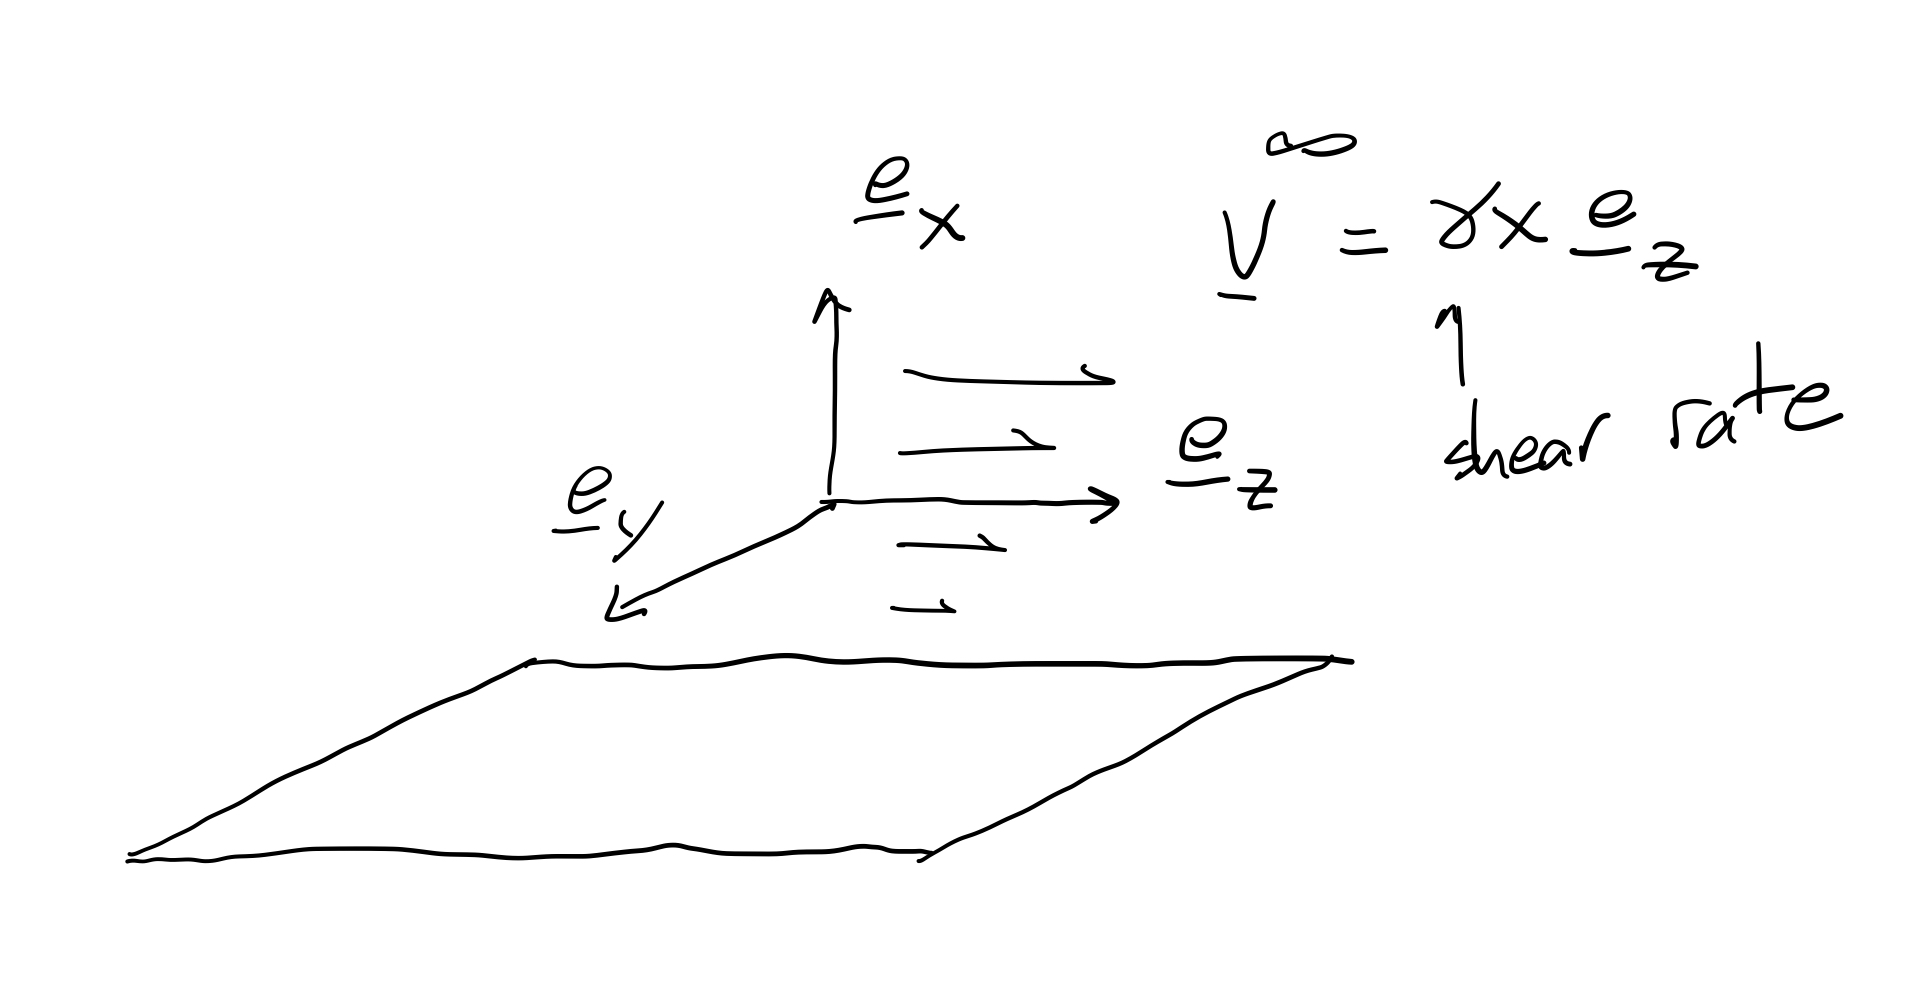
\includegraphics[width=\textwidth]{axes}
  \end{subfigure}
  \hfill
  \begin{subfigure}{0.49\textwidth}
    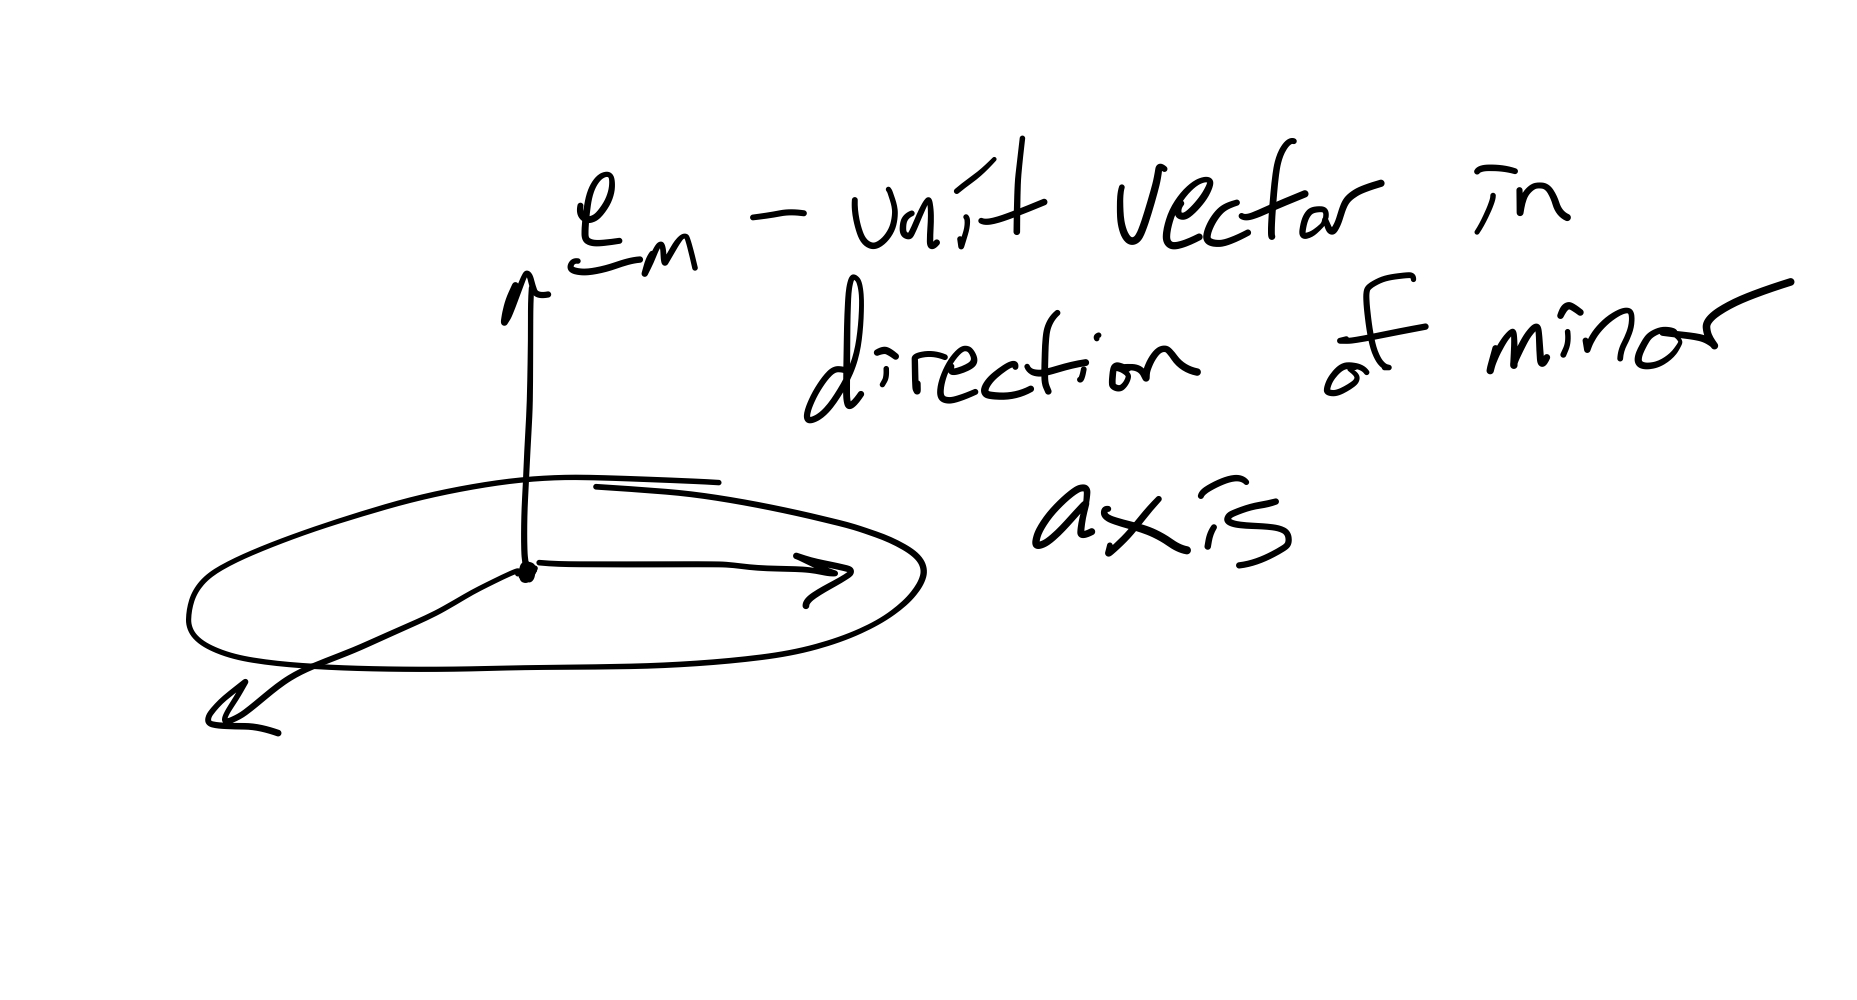
\includegraphics[width=\textwidth]{reference}
  \end{subfigure}
  \caption{Sketch of the axes and orientation angles of the ellipsoid}
  \label{fig:sketches}
\end{figure}

\textbf{Test Case: Sphere in an unbounded shear flow}

{\color{gray}
\begin{itemize}
\item The first test case I tried was a sphere in an unbounded shear
  flow. The velocity of the sphere in this case is $v_x = v_y = v_z =
  0$ (assuming $x = 0$), and the angular velocities are $\omega_x =
  \omega_z = 0$ and $\omega_y = -\gamma/2$.
\item Therefore with $\gamma = 1$,
  \textcolor{black}{$\dfrac{de_{m,x}}{dt} = -\dfrac{e_{m, z}}{2}$,
    $\dfrac{de_{m, y}}{dt} = 0$, and
    $\dfrac{de_{m,z}}{dt} = \dfrac{e_{m,x}}{2}$. These have the
    analytical solutions
    $\vect{e}_m = \frac{1}{2} (e_{m,x,0} \cos(t) - e_{m,z,0} \sin(t),
    e_{m,y,0}, e_{m,z,0} \cos(t) + e_{m,x,0}\sin(t))^T$.}
\item \textcolor{black}{Then I compared this analytic solution with
    the routine described above using regularized Stokeslets (results
    in Figure \ref{fig:com_plot})}
\item Note: in this test case, the regularized Stokeslets routine
  gives translational and angular velocities that are exact within
  machine precision (I don't really know why, perhaps because of
  symmetry we get mirrored errors that cancel each other out
  somehow). Therefore the error that is shown in Figure
  \ref{fig:com_plot} is only due to the Forward Euler integration. 
\end{itemize}
}

\begin{figure}
  \centering
  \begin{subfigure}{0.49\textwidth}
    \includegraphics[width=\textwidth]{com_plot1}
  \end{subfigure}
  \hfill
  \begin{subfigure}{0.49\textwidth}
    \includegraphics[width=\textwidth]{orient_plot1}
  \end{subfigure}
  \\
  \begin{subfigure}{0.49\textwidth}
    \includegraphics[width=\textwidth]{orient_err_plot1}
  \end{subfigure}
  \caption{Plots of the platelet position and orientation in an
    unbounded shear flow. Orientation is initialized at
    $\vect{e}_m = \vect{e}_x$.}
  \label{fig:com_plot}
\end{figure}

\newpage

\textbf{Test Case: Sphere in a shear flow, adjacent to a wall}

\begin{itemize}
\item For the second test case, place a sphere in a shear flow near a
  plane wall.
\item Goldman, Cox, and Brenner \cite{Goldman1967b} assemble results
  from an asymptotic approximation for the free motion of a sphere in
  this case (the approximation is valid in the limit
  $x \rightarrow a$, where $a$ is the radius of the sphere). The only
  nonzero components of the velocity are $v_z$ and $\omega_y$.
\item I experimented with different distances from the wall, and two
  different discretization sizes. I present my results below.
\end{itemize}

\emph{Experiments with different distances and 2 different mesh
  widths}

\begin{itemize}
\item I tried two different mesh sizes: 386 nodes, and 1538 nodes
  ($\approx 4\times$ more). The widths of these two meshes are
  $\approx 0.18$ and $\approx 0.09$, and the regularization parameter
  $\epsilon$ is chosen to be $\epsilon = 0.6 * h$, resulting in
  $\epsilon$ values of $0.108$ and $0.054$.
\item In the series of plots below, I plot the center of mass as a
  function of time, the components of the orientation vector
  $\vect{e}_m$, the error in each of the estimated $\vect{e}_m$
  components, and the error in the velocity estimate at each step. The
  error in the velocity is calculated as the max norm of the
  approximate 6D velocity vector minus the exact 6D velocity vector.
\item As the sphere is moved closer the to wall, the regularized
  Stokeslets cause the sphere to be ``sticky,'' in that the estimated
  translation velocity is slower than the analytic velocity, and the estimated
  angular velocity is higher than the analytic angular velocity.
\item Overall, as expected the accuracy gets worse as the sphere
  approaches the wall. However one weird result is that the fine mesh
  doesn't do any better than the coarse mesh at the smallest
  distance. I should revisit this to make sure this isn't the result
  of some bug.
\item At the larger distances, the error in the simulation with the
  fine grid is about 1/2 the error with the coarse grid, but when the
  distance to the wall is the same order as the blob size, the finer
  mesh doesn't do much better.
\end{itemize}

\begin{figure}
  \centering
  \begin{subfigure}{0.49\textwidth}
    \includegraphics[width=\textwidth]{com_plot2}
  \end{subfigure}
  \hfill
  \begin{subfigure}{0.49\textwidth}
    \includegraphics[width=\textwidth]{orient_plot2}
  \end{subfigure}
  \\
  \begin{subfigure}{0.49\textwidth}
    \includegraphics[width=\textwidth]{orient_err_plot2}
  \end{subfigure}
  \hfill
  \begin{subfigure}{0.49\textwidth}
    \includegraphics[width=\textwidth]{vel_err_plot2}
  \end{subfigure}
  \caption{Plots of the platelet position and orientation in a shear
    flow near a wall. Orientation is initialized at $\vect{e}_m =
    \vect{e}_x$.} 
  \label{fig:com_plot2}
\end{figure}

\begin{figure}
  \centering
  \begin{subfigure}{0.49\textwidth}
    \includegraphics[width=\textwidth]{com_plot3}
  \end{subfigure}
  \hfill
  \begin{subfigure}{0.49\textwidth}
    \includegraphics[width=\textwidth]{orient_plot3}
  \end{subfigure}
  \\
  \begin{subfigure}{0.49\textwidth}
    \includegraphics[width=\textwidth]{orient_err_plot3}
  \end{subfigure}
  \hfill
  \begin{subfigure}{0.49\textwidth}
    \includegraphics[width=\textwidth]{vel_err_plot3}
  \end{subfigure}
  \caption{Plots of the platelet position and orientation in a shear
    flow near a wall. Orientation is initialized at $\vect{e}_m =
    \vect{e}_x$.} 
  \label{fig:com_plot3}
\end{figure}

\begin{figure}
  \centering
  \begin{subfigure}{0.49\textwidth}
    \includegraphics[width=\textwidth]{com_plot4}
  \end{subfigure}
  \hfill
  \begin{subfigure}{0.49\textwidth}
    \includegraphics[width=\textwidth]{orient_plot4}
  \end{subfigure}
  \\
  \begin{subfigure}{0.49\textwidth}
    \includegraphics[width=\textwidth]{orient_err_plot4}
  \end{subfigure}
  \hfill
  \begin{subfigure}{0.49\textwidth}
    \includegraphics[width=\textwidth]{vel_err_plot4}
  \end{subfigure}
  \caption{Plots of the platelet position and orientation in a shear
    flow near a wall. Orientation is initialized at $\vect{e}_m =
    \vect{e}_x$.} 
  \label{fig:com_plot4}
\end{figure}

\begin{figure}
  \centering
  \begin{subfigure}{0.49\textwidth}
    \includegraphics[width=\textwidth]{com_plot5}
  \end{subfigure}
  \hfill
  \begin{subfigure}{0.49\textwidth}
    \includegraphics[width=\textwidth]{orient_plot5}
  \end{subfigure}
  \\
  \begin{subfigure}{0.49\textwidth}
    \includegraphics[width=\textwidth]{orient_err_plot5}
  \end{subfigure}
  \hfill
  \begin{subfigure}{0.49\textwidth}
    \includegraphics[width=\textwidth]{vel_err_plot5}
  \end{subfigure}
  \caption{Plots of the platelet position and orientation in a shear
    flow near a wall. Orientation is initialized at $\vect{e}_m =
    \vect{e}_x$.} 
  \label{fig:com_plot5}
\end{figure}

\begin{figure}
  \centering
  \begin{subfigure}{0.49\textwidth}
    \includegraphics[width=\textwidth]{com_plot6}
  \end{subfigure}
  \hfill
  \begin{subfigure}{0.49\textwidth}
    \includegraphics[width=\textwidth]{orient_plot6}
  \end{subfigure}
  \\
  \begin{subfigure}{0.49\textwidth}
    \includegraphics[width=\textwidth]{orient_err_plot6}
  \end{subfigure}
  \hfill
  \begin{subfigure}{0.49\textwidth}
    \includegraphics[width=\textwidth]{vel_err_plot6}
  \end{subfigure}
  \caption{Plots of the platelet position and orientation in a shear
    flow near a wall. Orientation is initialized at $\vect{e}_m =
    \vect{e}_x$.} 
  \label{fig:com_plot6}
\end{figure}

\begin{figure}
  \centering
  \begin{subfigure}{0.49\textwidth}
    \includegraphics[width=\textwidth]{com_plot7}
  \end{subfigure}
  \hfill
  \begin{subfigure}{0.49\textwidth}
    \includegraphics[width=\textwidth]{orient_plot7}
  \end{subfigure}
  \\
  \begin{subfigure}{0.49\textwidth}
    \includegraphics[width=\textwidth]{orient_err_plot7}
  \end{subfigure}
  \hfill
  \begin{subfigure}{0.49\textwidth}
    \includegraphics[width=\textwidth]{vel_err_plot7}
  \end{subfigure}
  \caption{Plots of the platelet position and orientation in a shear
    flow near a wall. Orientation is initialized at $\vect{e}_m =
    \vect{e}_x$.} 
  \label{fig:com_plot7}
\end{figure}

\begin{figure}
  \centering
  \begin{subfigure}{0.49\textwidth}
    \includegraphics[width=\textwidth]{com_plot8}
  \end{subfigure}
  \hfill
  \begin{subfigure}{0.49\textwidth}
    \includegraphics[width=\textwidth]{orient_plot8}
  \end{subfigure}
  \\
  \begin{subfigure}{0.49\textwidth}
    \includegraphics[width=\textwidth]{orient_err_plot8}
  \end{subfigure}
  \hfill
  \begin{subfigure}{0.49\textwidth}
    \includegraphics[width=\textwidth]{vel_err_plot8}
  \end{subfigure}
  \caption{Plots of the platelet position and orientation in a shear
    flow near a wall. Orientation is initialized at $\vect{e}_m =
    \vect{e}_x$.} 
  \label{fig:com_plot8}
\end{figure}

\begin{figure}
  \centering
  \begin{subfigure}{0.49\textwidth}
    \includegraphics[width=\textwidth]{com_plot9}
  \end{subfigure}
  \hfill
  \begin{subfigure}{0.49\textwidth}
    \includegraphics[width=\textwidth]{orient_plot9}
  \end{subfigure}
  \\
  \begin{subfigure}{0.49\textwidth}
    \includegraphics[width=\textwidth]{orient_err_plot9}
  \end{subfigure}
  \hfill
  \begin{subfigure}{0.49\textwidth}
    \includegraphics[width=\textwidth]{vel_err_plot9}
  \end{subfigure}
  \caption{Plots of the platelet position and orientation in a shear
    flow near a wall. Orientation is initialized at $\vect{e}_m =
    \vect{e}_x$.} 
  \label{fig:com_plot9}
\end{figure}

\bibliographystyle{plain}
\bibliography{/Users/andrewwork/Documents/grad-school/thesis/library}

\end{document}




